% !TEX program = xelatex
% ============================================================================
%  POSN Computer Qualification — Analytic Geometry & Vectors
%  Topic: เรขาคณิตวิเคราะห์และเวกเตอร์
% ============================================================================

\documentclass[11pt, aspectratio=169]{beamer}

% ============================================================================
%  POSN Computer Qualification — Shared Beamer Preamble
%  Used by all topic slide decks. Compile with XeLaTeX.
% ============================================================================

% ---------- Thai language & font ----------
\usepackage{iftex}
\usepackage{fontspec}

% XeTeX-specific: enable Thai line breaking
\ifXeTeX
  \XeTeXlinebreaklocale{th}
\fi
% Noto Sans Thai — body text (clean modern sans-serif, handles all Thai)
\setmainfont{Noto Sans Thai}[
  UprightFont = Noto Sans Thai Light,
  BoldFont    = Noto Sans Thai Medium,
  Scale       = 0.9
]
\setsansfont{Noto Sans Thai}[
  UprightFont = Noto Sans Thai Light,
  BoldFont    = Noto Sans Thai Medium,
  Scale       = 0.9
]

% Noto Sans Thai — clean modern sans-serif for structural elements
\newfontfamily\headingfont{Noto Sans Thai}[
  UprightFont = Noto Sans Thai Medium,
  BoldFont    = Noto Sans Thai Bold,
  Scale       = 0.9
]

% --- Heading font for structural elements ---
\setbeamerfont{title}{family=\headingfont, series=\bfseries, size=\huge}
\setbeamerfont{subtitle}{family=\headingfont, series=\mdseries}
\setbeamerfont{author}{family=\headingfont, series=\mdseries}

% --- Custom Title Page ---
\defbeamertemplate{title page}{custom}[1][]{%
  \centering
  \vspace*{2cm}
  % Title — in white
  {\usebeamerfont{title}\color{white}\inserttitle\par}
  \vspace{0.6cm}
  % Subtitle — in white
  {\usebeamerfont{subtitle}\color{white}\insertsubtitle\par}
  \vspace{2.5cm}
  % Author — blue filled rounded box, white text
  \begin{center}
    \begin{tcolorbox}[arc=3mm, colback=boxBlue, colframe=boxBlue!80,
                      width=0.42\textwidth, halign=center,
                      left=1.5em, right=1.5em, top=0.8em, bottom=0.8em,
                      boxrule=1.5pt, coltext=white]
      \usebeamerfont{author}\insertauthor
    \end{tcolorbox}
  \end{center}
}
\setbeamertemplate{title page}[custom]
\setbeamerfont{frametitle}{family=\headingfont, series=\bfseries}
\setbeamerfont{section in toc}{family=\headingfont}
\setbeamerfont{page number in head/foot}{family=\headingfont}
\setbeamerfont{section title}{family=\headingfont, series=\bfseries}
\setbeamerfont{subsection title}{family=\headingfont}

% Monospace font (for code/verbatim)
\setmonofont{Latin Modern Mono}[Scale=0.9]

% ---------- Math ----------
\usepackage{amsmath, amssymb}

% ---------- Graphics ----------
\usepackage{graphicx}
\usepackage{tikz}

% ---------- String parsing (for section headers) ----------
\usepackage{xstring}

% ---------- Colored boxes ----------
\usepackage[skins, breakable, xparse]{tcolorbox}
% Note: we do NOT load the 'most' option — it predefines example/solution environments
% that would conflict with our custom boxes.

% --- Color definitions ---
\definecolor{boxBlue}{RGB}{41, 128, 185}
\definecolor{boxGreen}{RGB}{39, 174, 96}
\definecolor{boxOrange}{RGB}{230, 126, 34}
\definecolor{boxPurple}{RGB}{142, 68, 173}
\definecolor{boxBlueBg}{RGB}{235, 245, 255}
\definecolor{boxGreenBg}{RGB}{235, 255, 240}
\definecolor{boxOrangeBg}{RGB}{255, 245, 235}
\definecolor{boxPurpleBg}{RGB}{248, 240, 255}

% --- Explanation box (blue) — for definitions, concepts, notes ---
\newtcolorbox{explanation}[1][]{
  enhanced,
  breakable,
  arc         = 2mm,
  colback     = boxBlueBg,
  colframe    = boxBlue!50,
  title       = #1,
  fonttitle   = \bfseries\color{white},
  coltitle    = white,
  colbacktitle= boxBlue,
  attach boxed title to top left = {yshift=-2mm, xshift=2mm},
  boxed title style = {arc=2mm, size=small},
  before skip = 8pt,
  after skip  = 8pt
}

% --- Example box (green) — for worked examples ---
\newtcolorbox{exambox}[1][]{
  enhanced,
  breakable,
  arc         = 2mm,
  colback     = boxGreenBg,
  colframe    = boxGreen!50,
  title       = #1,
  fonttitle   = \bfseries\color{white},
  coltitle    = white,
  colbacktitle= boxGreen,
  attach boxed title to top left = {yshift=-2mm, xshift=2mm},
  boxed title style = {arc=2mm, size=small},
  before skip = 8pt,
  after skip  = 8pt
}

% --- Solution box (orange) — for solutions and answers ---
\newtcolorbox{solbox}[1][]{
  enhanced,
  breakable,
  arc         = 2mm,
  colback     = boxOrangeBg,
  colframe    = boxOrange!50,
  title       = #1,
  fonttitle   = \bfseries\color{white},
  coltitle    = white,
  colbacktitle= boxOrange,
  attach boxed title to top left = {yshift=-2mm, xshift=2mm},
  boxed title style = {arc=2mm, size=small},
  before skip = 8pt,
  after skip  = 8pt
}

% --- Intuition box (purple) — for plain-language explanations, analogies ---
\newtcolorbox{intuition}[1][]{
  enhanced,
  breakable,
  arc         = 2mm,
  colback     = boxPurpleBg,
  colframe    = boxPurple!50,
  title       = #1,
  fonttitle   = \bfseries\color{white},
  coltitle    = white,
  colbacktitle= boxPurple,
  attach boxed title to top left = {yshift=-2mm, xshift=2mm},
  boxed title style = {arc=2mm, size=small},
  before skip = 8pt,
  after skip  = 8pt
}

% ---------- Beamer theme ----------
\usetheme{Madrid}
\usecolortheme{default}

% --- Custom beamer colors (blue accent matching explanation boxes) ---
\setbeamercolor{structure}{fg=boxBlue}
\setbeamercolor{palette primary}{fg=white, bg=boxBlue}
\setbeamercolor{palette secondary}{fg=white, bg=boxBlue!80}
\setbeamercolor{palette tertiary}{fg=white, bg=boxBlue!60}
\setbeamercolor{block title}{fg=white, bg=boxBlue}
\setbeamercolor{block body}{fg=black, bg=boxBlueBg}

% Remove navigation symbols for clean look
\setbeamertemplate{navigation symbols}{}

% Note: Frame title prefix removed — \addtobeamertemplate conflicts with beamer internals

% --- Outline (Table of Contents) styling ---
\setbeamerfont{section in toc}{family=\headingfont, series=\mdseries}
\setbeamerfont{subsection in toc}{family=\headingfont, series=\mdseries}
\setbeamertemplate{section in toc}{%
  \leavevmode\leftskip=1.5em
  \textcolor{boxBlue}{\textbf{\large\inserttocsectionnumber.}}%
  \quad\inserttocsection\par
  \vspace{0.2em}
}
\setbeamertemplate{subsection in toc}{%
  \leavevmode\leftskip=4em
  \textcolor{boxBlue!60}{\small$\bullet$}%
  \quad\inserttocsubsection\par
  \vspace{0.1em}
}

% Section header slides — Thai in white, English in smaller light blue below
\AtBeginSection{
  \begin{frame}[plain]{}
    \vspace*{2cm}
    \begin{beamercolorbox}[sep=12pt, center, rounded=true, shadow=true]{palette primary}
      \IfSubStr{\secname}{(}{%
        \StrBefore{\secname}{(}[\sectionthai]%
        \StrBetween[1,1]{\secname}{(}{)}[\sectioneng]%
        \begin{tabular}{@{}c@{}}
          {\usebeamerfont{title}\sectionthai} \\[0.2em]
          {\usebeamerfont{subtitle}\color{boxBlue!60}\sectioneng}
        \end{tabular}%
      }{%
        {\usebeamerfont{title}\secname\par}%
      }
    \end{beamercolorbox}
    \vfill
  \end{frame}
}

% Subsection header slides — smaller, centered
\AtBeginSubsection{
  \begin{frame}[plain]{}
    \vfill
    \centering
    {\usebeamerfont{section title}\insertsubsectionhead\par}
    \vfill
  \end{frame}
}

% Minimal footer: page number only, right-aligned
\setbeamertemplate{footline}{
  \hfill\usebeamerfont{page number in head/foot}\insertframenumber{} / \inserttotalframenumber\hspace*{1em}\vspace*{0.5ex}
}

% ---------- Spacing & readability ----------
\linespread{1.2}

% ---------- Useful commands ----------

% Highlight important text in blue
\newcommand{\highlight}[1]{\textcolor{boxBlue}{\textbf{#1}}}

% Math set notation helpers
\newcommand{\R}{\mathbb{R}}
\newcommand{\N}{\mathbb{N}}
\newcommand{\Z}{\mathbb{Z}}
\newcommand{\Q}{\mathbb{Q}}

% ============================================================================
%  End of preamble
% ============================================================================


\title[เรขาคณิตวิเคราะห์]{เรขาคณิตวิเคราะห์และเวกเตอร์}
\subtitle{Analytic Geometry \& Vectors — ระนาบพิกัด, ระยะทาง, ความชัน, เส้นตรง, มุม, เวกเตอร์}
\author[None W. (Yuan)]{None W. (Yuan)}
\date{}

\begin{document}

\begin{frame}[plain]\titlepage\end{frame}
\begin{frame}{สารบัญ (Outline)}\tableofcontents\end{frame}

\begin{frame}{ก่อนเรียน (Prerequisites)}
  \begin{explanation}[สิ่งที่ควรรู้ก่อนเรียน]
    \begin{itemize}
      \item \textbf{จำนวนจริง} — การดำเนินการพื้นฐาน, รากที่สอง, ค่าสัมบูรณ์
      \item \textbf{สมการ} — การแก้สมการเชิงเส้น, การจัดรูปสมการ
    \end{itemize}
  \end{explanation}

  \begin{intuition}[เรขาคณิตวิเคราะห์คืออะไร?]
    การนำ \highlight{พีชคณิต} มาใช้กับ \highlight{เรขาคณิต}
    — ใช้พิกัดและสมการอธิบายรูปเรขาคณิต
  \end{intuition}
\end{frame}

% ===========================================================================
%  SECTION 1: ระบบพิกัดฉาก
% ===========================================================================
\section{ระบบพิกัดฉาก (Coordinate System)}

\begin{frame}{ระนาบพิกัด (Coordinate Plane)}
  \begin{explanation}[องค์ประกอบ]
    \begin{itemize}
      \item \textbf{แกนนอน} ($x$-axis) และ \textbf{แกนตั้ง} ($y$-axis)
      \item \textbf{จุดกำเนิด} $O(0, 0)$ — จุดตัดของสองแกน
      \item \textbf{จุด} $(x, y)$ — บอกตำแหน่งบนระนาบ ($x$ = แกนนอน, $y$ = แกนตั้ง)
      \item ระนาบแบ่งออกเป็น 4 จตุภาค (Quadrants I, II, III, IV)
    \end{itemize}
  \end{explanation}
\end{frame}

\begin{frame}{ระนาบพิกัด — ตัวอย่าง}
  \centering
  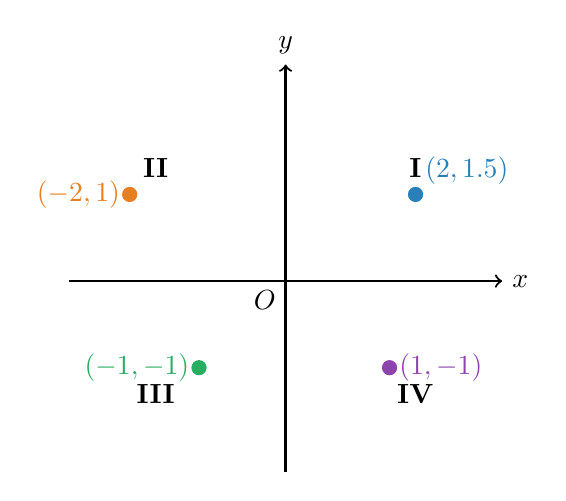
\begin{tikzpicture}[scale=1.1]
    \draw[->, thick] (-2.5,0) -- (2.5,0) node[right] {$x$};
    \draw[->, thick] (0,-2.2) -- (0,2.5) node[above] {$y$};
    \node at (0,0) [below left] {$O$};
    \node at (1.5,1.3) {\textbf{I}};
    \node at (-1.5,1.3) {\textbf{II}};
    \node at (-1.5,-1.3) {\textbf{III}};
    \node at (1.5,-1.3) {\textbf{IV}};

    \fill[boxBlue] (1.5,1) circle (2.5pt) node[above right] {$(2,1.5)$};
    \fill[boxOrange] (-1.8,1) circle (2.5pt) node[left] {$(-2,1)$};
    \fill[boxGreen] (-1,-1) circle (2.5pt) node[left] {$(-1,-1)$};
    \fill[boxPurple] (1.2,-1) circle (2.5pt) node[right] {$(1,-1)$};
  \end{tikzpicture}
\end{frame}

% ===========================================================================
%  SECTION 2: ระยะทางและจุดกึ่งกลาง
% ===========================================================================
\section{ระยะทางและจุดกึ่งกลาง (Distance \& Midpoint)}

\begin{frame}{ระยะทางระหว่างจุดสองจุด}
  \begin{explanation}[สูตรระยะทาง] (มาจากทฤษฎีบทพีทาโกรัส!)
    ระยะทางระหว่าง $P_1(x_1, y_1)$ และ $P_2(x_2, y_2)$:
    \[
      d = \sqrt{(x_2 - x_1)^2 + (y_2 - y_1)^2}
    \]
  \end{explanation}

  \centering
  \begin{tikzpicture}[scale=1.1]
    \draw[->, gray] (-0.5,0) -- (4.5,0) node[right] {$x$};
    \draw[->, gray] (0,-0.5) -- (0,3.5) node[above] {$y$};
    \fill[boxBlue] (1,1) circle (2pt) node[below left] {$P_1$};
    \fill[boxBlue] (3.5,2.8) circle (2pt) node[above right] {$P_2$};
    \draw[boxBlue, thick] (1,1) -- (3.5,2.8);
    \draw[dashed, boxOrange] (1,1) -- (3.5,1) node[midway, below] {$\Delta x$};
    \draw[dashed, boxGreen] (3.5,1) -- (3.5,2.8) node[midway, right] {$\Delta y$};
  \end{tikzpicture}
\end{frame}

\begin{frame}{ตัวอย่าง: ระยะทาง}
  \begin{exambox}[โจทย์ 1]
    ระยะทางระหว่าง $A(2,3)$ และ $B(5,7)$
    
    \medskip
    $d = \sqrt{(5-2)^2 + (7-3)^2}
        = \sqrt{3^2 + 4^2}
        = \sqrt{9 + 16} = 5$
  \end{exambox}
\end{frame}

\begin{frame}{ตัวอย่าง: ระยะทาง (ต่อ)}
  \begin{exambox}[โจทย์ 2]
    ระยะทางระหว่าง $C(-1,2)$ และ $D(3,-1)$ 

    \medskip
    $d = \sqrt{(3-(-1))^2 + (-1-2)^2}
        = \sqrt{4^2 + (-3)^2}
        = \sqrt{16 + 9} = 5$
  \end{exambox}

  \begin{intuition}[สังเกต]
    ระยะทางระหว่าง $A$ ถึง $B$ และ $C$ ถึง $D$ เท่ากัน ($= 5$)
    แต่คู่ของจุดอยู่คนละตำแหน่ง — ระยะทางขึ้นกับ \highlight{ผลต่าง} ของพิกัดเท่านั้น
  \end{intuition}
\end{frame}

\begin{frame}{จุดกึ่งกลาง (Midpoint)}
  \begin{explanation}[สูตรจุดกึ่งกลาง]
    จุดกึ่งกลาง $M$ ระหว่าง $P_1(x_1, y_1)$ และ $P_2(x_2, y_2)$:
    \[
      M = \left(\frac{x_1 + x_2}{2},\; \frac{y_1 + y_2}{2}\right)
    \]
  \end{explanation}

  \centering
  \begin{tikzpicture}[scale=0.8]
    \draw[->, gray] (-0.5,0) -- (4.5,0) node[right] {$x$};
    \draw[->, gray] (0,-0.5) -- (0,3.5) node[above] {$y$};
    \fill[boxBlue] (1,1) circle (2pt) node[below] {$P_1$};
    \fill[boxBlue] (3.5,2.8) circle (2pt) node[above] {$P_2$};
    \fill[boxOrange] (2.25,1.9) circle (2.5pt) node[below right] {$M$};
    \draw[boxBlue, thick] (1,1) -- (3.5,2.8);
  \end{tikzpicture}

  % \begin{exambox}[ตัวอย่าง]
  %   $P_1(1,3)$, $P_2(5,7)$ \quad $\rightarrow$ \quad
  %   $M = \left(\frac{1+5}{2}, \frac{3+7}{2}\right) = (3, 5)$
  % \end{exambox}
\end{frame}

\begin{frame}{ตัวอย่าง: จุดกึ่งกลาง}
  \begin{exambox}[โจทย์]
    จงหาจุดกึ่งกลางระหว่าง $A(-2, 4)$ และ $B(6, -2)$
  \end{exambox}

  \begin{solbox}[วิธีทำ]
    $M = \left(\dfrac{-2+6}{2}, \dfrac{4+(-2)}{2}\right) = (2, 1)$
  \end{solbox}
\end{frame}

% ===========================================================================
%  SECTION 3: ความชันและมุม
% ===========================================================================
\section{ความชันและมุม (Slope \& Angle)}

\begin{frame}{ความชันของเส้นตรง (Slope)}
  \begin{explanation}[นิยาม]
    \textbf{ความชัน} $m$ ของเส้นตรงที่ผ่าน $P_1(x_1,y_1)$ และ $P_2(x_2,y_2)$:
    \[
      m = \frac{y_2 - y_1}{x_2 - x_1} = \frac{\text{การเปลี่ยนแปลงในแนวตั้ง}}{\text{การเปลี่ยนแปลงในแนวนอน}}
    \]
    (เมื่อ $x_1 \neq x_2$)
  \end{explanation}

  \begin{columns}[T]
    \column{0.25\textwidth}
      \centering
      \textbf{บวก} \quad $m > 0$ \\[0.5em]
      \begin{tikzpicture}[scale=0.7]
        \draw[->, gray] (-1.5,0)--(1.5,0); \draw[->, gray] (0,-1)--(0,1.5);
        \draw[boxBlue, thick] (-1,-0.5) -- (1,1);
      \end{tikzpicture}
    \column{0.25\textwidth}
      \centering
      \textbf{ลบ} \quad $m < 0$ \\[0.5em]
      \begin{tikzpicture}[scale=0.7]
        \draw[->, gray] (-1.5,0)--(1.5,0); \draw[->, gray] (0,-1)--(0,1.5);
        \draw[boxOrange, thick] (-1,1) -- (1,-0.5);
      \end{tikzpicture}
    \column{0.25\textwidth}
      \centering
      \textbf{ศูนย์} \quad $m = 0$ \\[0.5em]
      \begin{tikzpicture}[scale=0.7]
        \draw[->, gray] (-1.5,0)--(1.5,0); \draw[->, gray] (0,-1)--(0,1.5);
        \draw[boxGreen, thick] (-1.3,0.8) -- (1.3,0.8);
      \end{tikzpicture}
    \column{0.25\textwidth}
      \centering
      \textbf{ไม่นิยาม} \\[0.5em]
      \begin{tikzpicture}[scale=0.7]
        \draw[->, gray] (-1.5,0)--(1.5,0); \draw[->, gray] (0,-1)--(0,1.5);
        \draw[boxPurple, thick] (0.8,-0.8) -- (0.8,1.3);
      \end{tikzpicture}
  \end{columns}
\end{frame}

\begin{frame}{มุมระหว่างเส้นตรง (Angle Between Lines)}
  \begin{explanation}[สูตรมุมระหว่างเส้นตรงสองเส้น]
    ให้ $m_1, m_2$ เป็นความชันของเส้นตรงสองเส้น ($m_1m_2 \neq -1$):
    \[
      \tan \theta = \left|\frac{m_1 - m_2}{1 + m_1m_2}\right|
    \]
  \end{explanation}

  \begin{explanation}[เส้นขนานและเส้นตั้งฉาก]
    \begin{itemize}
      \item \textbf{ขนาน:} $m_1 = m_2$ \quad (มุมระหว่างเส้น $= 0^\circ$)
      \item \textbf{ตั้งฉาก:} $m_1 \cdot m_2 = -1$ \quad (มุมระหว่างเส้น $= 90^\circ$)
    \end{itemize}
  \end{explanation}
\end{frame}

\begin{frame}{ตัวอย่าง}
  \begin{exambox}[ตัวอย่าง: เส้นตั้งฉาก]
    เส้นที่ 1 มีความชัน $m_1 = 2$

    เส้นตั้งฉากต้องมีความชัน $m_2 = -\frac{1}{2}$

    เพราะ $2 \times (-\frac{1}{2}) = -1$ \quad $\checkmark$
  \end{exambox}

  \begin{exambox}[โจทย์]
    เส้นตรงที่ผ่าน $(1,2)$ และตั้งฉากกับ $y = 2x + 1$
    ความชันของเส้นที่ต้องการ $= -\frac{1}{2}$

    ใช้ point-slope: $y - 2 = -\frac{1}{2}(x - 1)$

    $y = -\frac{1}{2}x + \frac{5}{2}$
  \end{exambox}
\end{frame}

% ===========================================================================
%  SECTION 4: สมการเส้นตรง
% ===========================================================================
\section{สมการเส้นตรง (Equations of Lines)}

\begin{frame}{รูปแบบของสมการเส้นตรง}
  \begin{explanation}[รูปแบบ Point-Slope]
    เส้นตรงที่ผ่าน $(x_1, y_1)$ ด้วยความชัน $m$:
    \[
      y - y_1 = m(x - x_1)
    \]
  \end{explanation}

  \begin{explanation}[รูปแบบ Slope-Intercept]
    \[
      y = mx + c
    \]
    $m$ = ความชัน, \quad $c$ = ระยะตัดแกน $y$ (เมื่อ $x = 0$)
  \end{explanation}
\end{frame}

\begin{frame}{รูปแบบของสมการเส้นตรง}
  \begin{explanation}[รูปแบบทั่วไป (General Form)]
    \[
      Ax + By + C = 0
    \]
    โดยที่ $A, B, C$ เป็นค่าคงที่ และ $A, B$ ไม่เป็นศูนย์พร้อมกัน
  \end{explanation}
\end{frame}

\begin{frame}{ตัวอย่าง: การหาสมการเส้นตรง}
  \begin{exambox}[โจทย์]
    เส้นตรงผ่าน $(2, 3)$ และ $(4, 7)$
    \textbf{1. หาความชัน:}
    $m = \dfrac{7-3}{4-2} = \dfrac{4}{2} = 2$

    \textbf{2. ใช้ point-slope กับจุด $(2, 3)$:}
    $y - 3 = 2(x - 2)$
    $y - 3 = 2x - 4$

    \textbf{3. จัดรูป Slope-Intercept:}
    $y = 2x - 1$
  \end{exambox}
\end{frame}

\begin{frame}{กราฟของ $y = 2x - 1$}
  \centering
  \begin{tikzpicture}[scale=0.6]
    \draw[->, gray] (-1,0) -- (5,0) node[right] {$x$};
    \draw[->, gray] (0,-2) -- (0,7) node[above] {$y$};
    \draw[boxBlue, thick] (-0.5,-2) -- (4,7);
    \fill[boxBlue] (2,3) circle (2pt) node[below] {$(2,3)$};
    \fill[boxBlue] (4,7) circle (2pt) node[right] {$(4,7)$};
    \fill[boxOrange] (0,-1) circle (2pt) node[below right] {$c=-1$};
  \end{tikzpicture}

  เส้นตัดแกน $y$ ที่ $c = -1$, \; ความชัน $m = 2$
\end{frame}

\begin{frame}{ตัวอย่าง: การหาสมการเส้นตรง (ต่อ)}
  \begin{exambox}[โจทย์]
    เส้นตรงขนานกับ $y = 3x + 2$ และผ่าน $(0, 5)$
    ความชันเท่ากัน: $m = 3$

    ผ่าน $(0,5)$ — ระยะตัดแกน $y = 5$

    \textbf{คำตอบ:} $y = 3x + 5$
  \end{exambox}

  \begin{exambox}[โจทย์]
    เส้นตรงตั้งฉากกับ $y = \frac{1}{3}x - 1$ และผ่าน $(1, 2)$
    $m_{\text{ตั้งฉาก}} = -3$

    $y - 2 = -3(x - 1)$

    $y = -3x + 5$
  \end{exambox}
\end{frame}

% ===========================================================================
%  SECTION 5: เวกเตอร์
% ===========================================================================
\section{เวกเตอร์ (Vectors)}

\begin{frame}{เวกเตอร์คืออะไร?}
  \begin{explanation}[นิยาม]
    \textbf{เวกเตอร์} คือปริมาณที่มีทั้ง \highlight{ขนาด} และ \highlight{ทิศทาง}
    เขียนแทนด้วย $\vec{v}$ หรือลูกศรจากจุดเริ่มไปจุดปลาย
  \end{explanation}

  \begin{columns}[T]
    \column{0.5\textwidth}
      \centering
      \begin{tikzpicture}[scale=1.2]
        \draw[->, gray] (-0.5,0)--(3,0) node[right] {$x$};
        \draw[->, gray] (0,-0.5)--(0,2.5) node[above] {$y$};
        \draw[->, boxBlue, ultra thick] (0.0,0.0) -- (2.0,1.5)
          node[midway, above left] {$\vec{v} = (2, 1.5)$};
        \fill[boxBlue] (0,0) circle (1pt);
        \fill[boxBlue] (2,1.5) circle (1pt);
      \end{tikzpicture}

    \column{0.5\textwidth}
      \textbf{การเขียนเวกเตอร์:}
      \begin{itemize}
        \item $\vec{v} = (x, y)$ — พิกัด
        \item \textbf{ขนาด:} $|\vec{v}| = \sqrt{x^2 + y^2}$
        \item \textbf{ทิศทาง:} มุมจากแกน $x$ บวก
      \end{itemize}
  \end{columns}
\end{frame}

\begin{frame}{การดำเนินการของเวกเตอร์}
  \begin{explanation}[การบวกเวกเตอร์]
    $\vec{u} + \vec{v} = (u_1 + v_1,\; u_2 + v_2)$

    (นำพิกัดที่ตรงกันมาบวกกัน)
  \end{explanation}

  \begin{explanation}[การคูณด้วยสเกลาร์]
    $k\vec{v} = (k \cdot v_1,\; k \cdot v_2)$

    \begin{itemize}
      \item $k > 0$: เวกเตอร์ยาวขึ้นในทิศทางเดิม
      \item $k < 0$: เวกเตอร์ยาวขึ้นในทิศทางตรงข้าม
    \end{itemize}
  \end{explanation}

  \begin{exambox}[ตัวอย่าง]
    $\vec{u} = (3, 1)$, $\vec{v} = (-1, 2)$

    $\vec{u} + \vec{v} = (2, 3)$ \qquad $2\vec{u} = (6, 2)$
  \end{exambox}
\end{frame}

\begin{frame}{เวกเตอร์กับระยะทาง}
  \begin{explanation}[ระยะทางแบบยุคลีเดียน (Euclidean Distance)]
    ระยะทางระหว่าง $\vec{a}$ และ $\vec{b}$ = ขนาดของ $\vec{a} - \vec{b}$:
    \[
      d = |\vec{a} - \vec{b}| = \sqrt{(a_1-b_1)^2 + (a_2-b_2)^2}
    \]
    (เหมือนกับสูตรระยะทางระหว่างสองจุด!)
  \end{explanation}

  \begin{exambox}[ตัวอย่าง]
    $\vec{a} = (1, 2)$, $\vec{b} = (4, 6)$

    $\vec{a} - \vec{b} = (-3, -4)$

    $d = \sqrt{(-3)^2 + (-4)^2} = \sqrt{9 + 16} = 5$
  \end{exambox}
\end{frame}

% ===========================================================================
%  SUMMARY
% ===========================================================================
\section{สรุป}

\begin{frame}{สรุปเนื้อหา}
  \begin{explanation}[สิ่งที่ได้เรียนรู้]
    \begin{enumerate}
      \item \textbf{ระยะทาง}: $d = \sqrt{(x_2-x_1)^2 + (y_2-y_1)^2}$
      \item \textbf{จุดกึ่งกลาง}: $M = \left(\frac{x_1+x_2}{2}, \frac{y_1+y_2}{2}\right)$
      \item \textbf{ความชัน}: $m = \frac{y_2-y_1}{x_2-x_1}$, \; ขนาน $m_1=m_2$, \; ตั้งฉาก $m_1m_2=-1$
      \item \textbf{มุมระหว่างเส้น}: $\tan\theta = \left|\frac{m_1-m_2}{1+m_1m_2}\right|$
      \item \textbf{สมการเส้นตรง}: Point-slope, Slope-Intercept, General Form
      \item \textbf{เวกเตอร์}: $\vec{v} = (x,y)$, $|\vec{v}| = \sqrt{x^2+y^2}$, การบวก, สเกลาร์คูณ
    \end{enumerate}
  \end{explanation}
  \begin{center}
    \large เอกสารนี้เป็นส่วนหนึ่งของเนื้อหาเตรียมสอบ \textbf{สอวน. คอมพิวเตอร์}
  \end{center}
\end{frame}

\end{document}
